%----------------------------------------------------------------------------------------
%    PAGE ADJUSTMENTS
%----------------------------------------------------------------------------------------

\documentclass[12pt,a4paper,hidelinks]{article}            % Article 12pt font for a4 paper while hiding links
\usepackage[margin=1in]{geometry}                          % Required to adjust margins

%----------------------------------------------------------------------------------------
%    TYPE SETTING PACKAGES
%----------------------------------------------------------------------------------------

\usepackage[english]{babel}                                % English language/hyphenation 
\usepackage[utf8x]{inputenc}                               % Accept different input encodings
\usepackage{amsmath,amsfonts,amsthm,amssymb}               % Math packages to use equations
\usepackage{siunitx}                                       % Scientific units and numbering
\usepackage[usenames,dvipsnames,svgnames,table]{xcolor}    % Set color of text/background
\linespread{1.2}                                           % Default line spacing size
\usepackage{microtype}                                     % Improves spacing in the document
\usepackage{setspace}                                      % Set line spacing dynamically
\usepackage{tocloft}                                       % List adjustments including ToC
\usepackage{tikz}
\usepackage{caption}

%----------------------------------------------------------------------------------------
%    FIGURES
%----------------------------------------------------------------------------------------

\usepackage{graphicx}                                      % Required for the inclusion of images
\graphicspath{{./Pictures/}}                               % Specifies picture directory
\usepackage{float}                                         % Allows putting an [H] in \begin{figure}
\usepackage{wrapfig}                                       % Allows in-line images

\usepackage{hyperref}                                      % References
\usepackage{cleveref}                                      % Better References
%\crefname{lstlisting}{listing}{listings}
%\Crefname{lstlisting}{Listing}{Listings}
\crefname{figure}{figure}{figures}
\Crefname{figure}{Figure}{Figures}

%----------------------------------------------------------------------------------------
%    INCLUDE CODE
%----------------------------------------------------------------------------------------

\usepackage{listings}                                      % Package so code looks pretty
\lstset{
language=C,                                                % Choose the language
basicstyle=\footnotesize,                                  % The size of the fonts used
numbers=left,                                              % Where to put the line-numbers
numberstyle=\footnotesize,                                 % The size of the line-numbers
stepnumber=1,                                              % The step line-numbers
numbersep=5pt,                                             % How far the line-numbers are from the code
backgroundcolor=\color{white},                             % Choose the background color
showspaces=false,                                          % Show spaces adding partiular underscores
showstringspaces=false,                                    % Underline spaces within strings
showtabs=false,                                            % Show tabs within strings adding particular underscores
frame=single,                                              % Adds a frame around the code
tabsize=2,                                                 % Sets default tabsize to 2 spaces
captionpos=b,                                              % Sets the caption-position to bottom
breaklines=true,                                           % Sets automatic line breaking
breakatwhitespace=false,                                   % Sets if automatic breaks should only happen at whitespace
escapeinside={\%*}{*)}                                     % If you want to add a comment within your code
}

%----------------------------------------------------------------------------------------
%    EXTRAS
%----------------------------------------------------------------------------------------

\usepackage{attachfile}                                    % Attach files to your document
\usepackage{fancyhdr}                                      % Fancy Header

\begin{document}

%----------------------------------------------------------------------------------------
%    COMMANDS
%----------------------------------------------------------------------------------------

\setlength\parindent{0pt}                                  % Removes all indentation from paragraphs
\renewcommand*\thesection{\arabic{section}}                % Renew section numbers
\renewcommand{\labelenumi}{\alph{enumi}.}                  % Section ordered numbering
\let\oldvec\vec                                            % Save the old vector style
\renewcommand{\vec}[1]{\oldvec{\mathbf{#1}}}               % Set vectors to look like vectors

\renewcommand{\contentsname}{Table of Contents}            % Make ToC actually say ToC
\addtocontents{toc}{~\hfill\textbf{Page}\par}              % Add 'page' to top of ToC
\renewcommand{\cftsecleader}{\cftdotfill{\cftdotsep}}      % Makes dots leading up to page number
\setcounter{tocdepth}{3}                                   % Depth of ToC
\setcounter{lofdepth}{3}                                   % Depth of LoF

\pagestyle{fancy}                                          % Fancy page style for headers
\setlength{\headheight}{15pt}                              % Change header hieght
\fancyhead[L,LO]{\fontsize{8}{10} \selectfont \firstmark}  % Adds header to left with section name
\fancyhead[R,RO]{\fontsize{8}{10} \selectfont Seth Miers}  % Adds header to right
\definecolor{grey}{HTML}{cccccc}                           % The next 4 lines modifies the header (color)
\renewcommand{\headrulewidth}{1px}
\renewcommand{\headrule}{{\color{grey}%
\hrule width\headwidth height\headrulewidth%
\vskip-\headrulewidth}}

\numberwithin{equation}{section}                           % Number equations within sections
\numberwithin{figure}{section}                             % Number figures within sections
\numberwithin{table}{section}                              % Number tables within sections
\numberwithin{lstlisting}{section}                         % Number listings within sections

\renewcommand{\sfdefault}{phv}                             % Change default font
\renewcommand{\familydefault}{\sfdefault}                  % Use default font everywhere

%----------------------------------------------------------------------------------------
%    TITLE PAGE
%----------------------------------------------------------------------------------------

\begin{titlepage}

\title{Real Time Clock}
\author{Seth Miers}

\vspace*{\fill}                                            % Center title page vertically

\newcommand{\HRule}{\rule{\linewidth}{0.3mm}}              % Defines horizontal lines

\center                                                    % Center everything on the page

\textsc{\LARGE University of Colorado}\\[1.5cm]            % First heading

\vspace{-3em}

\begin{figure}[H]
\centering
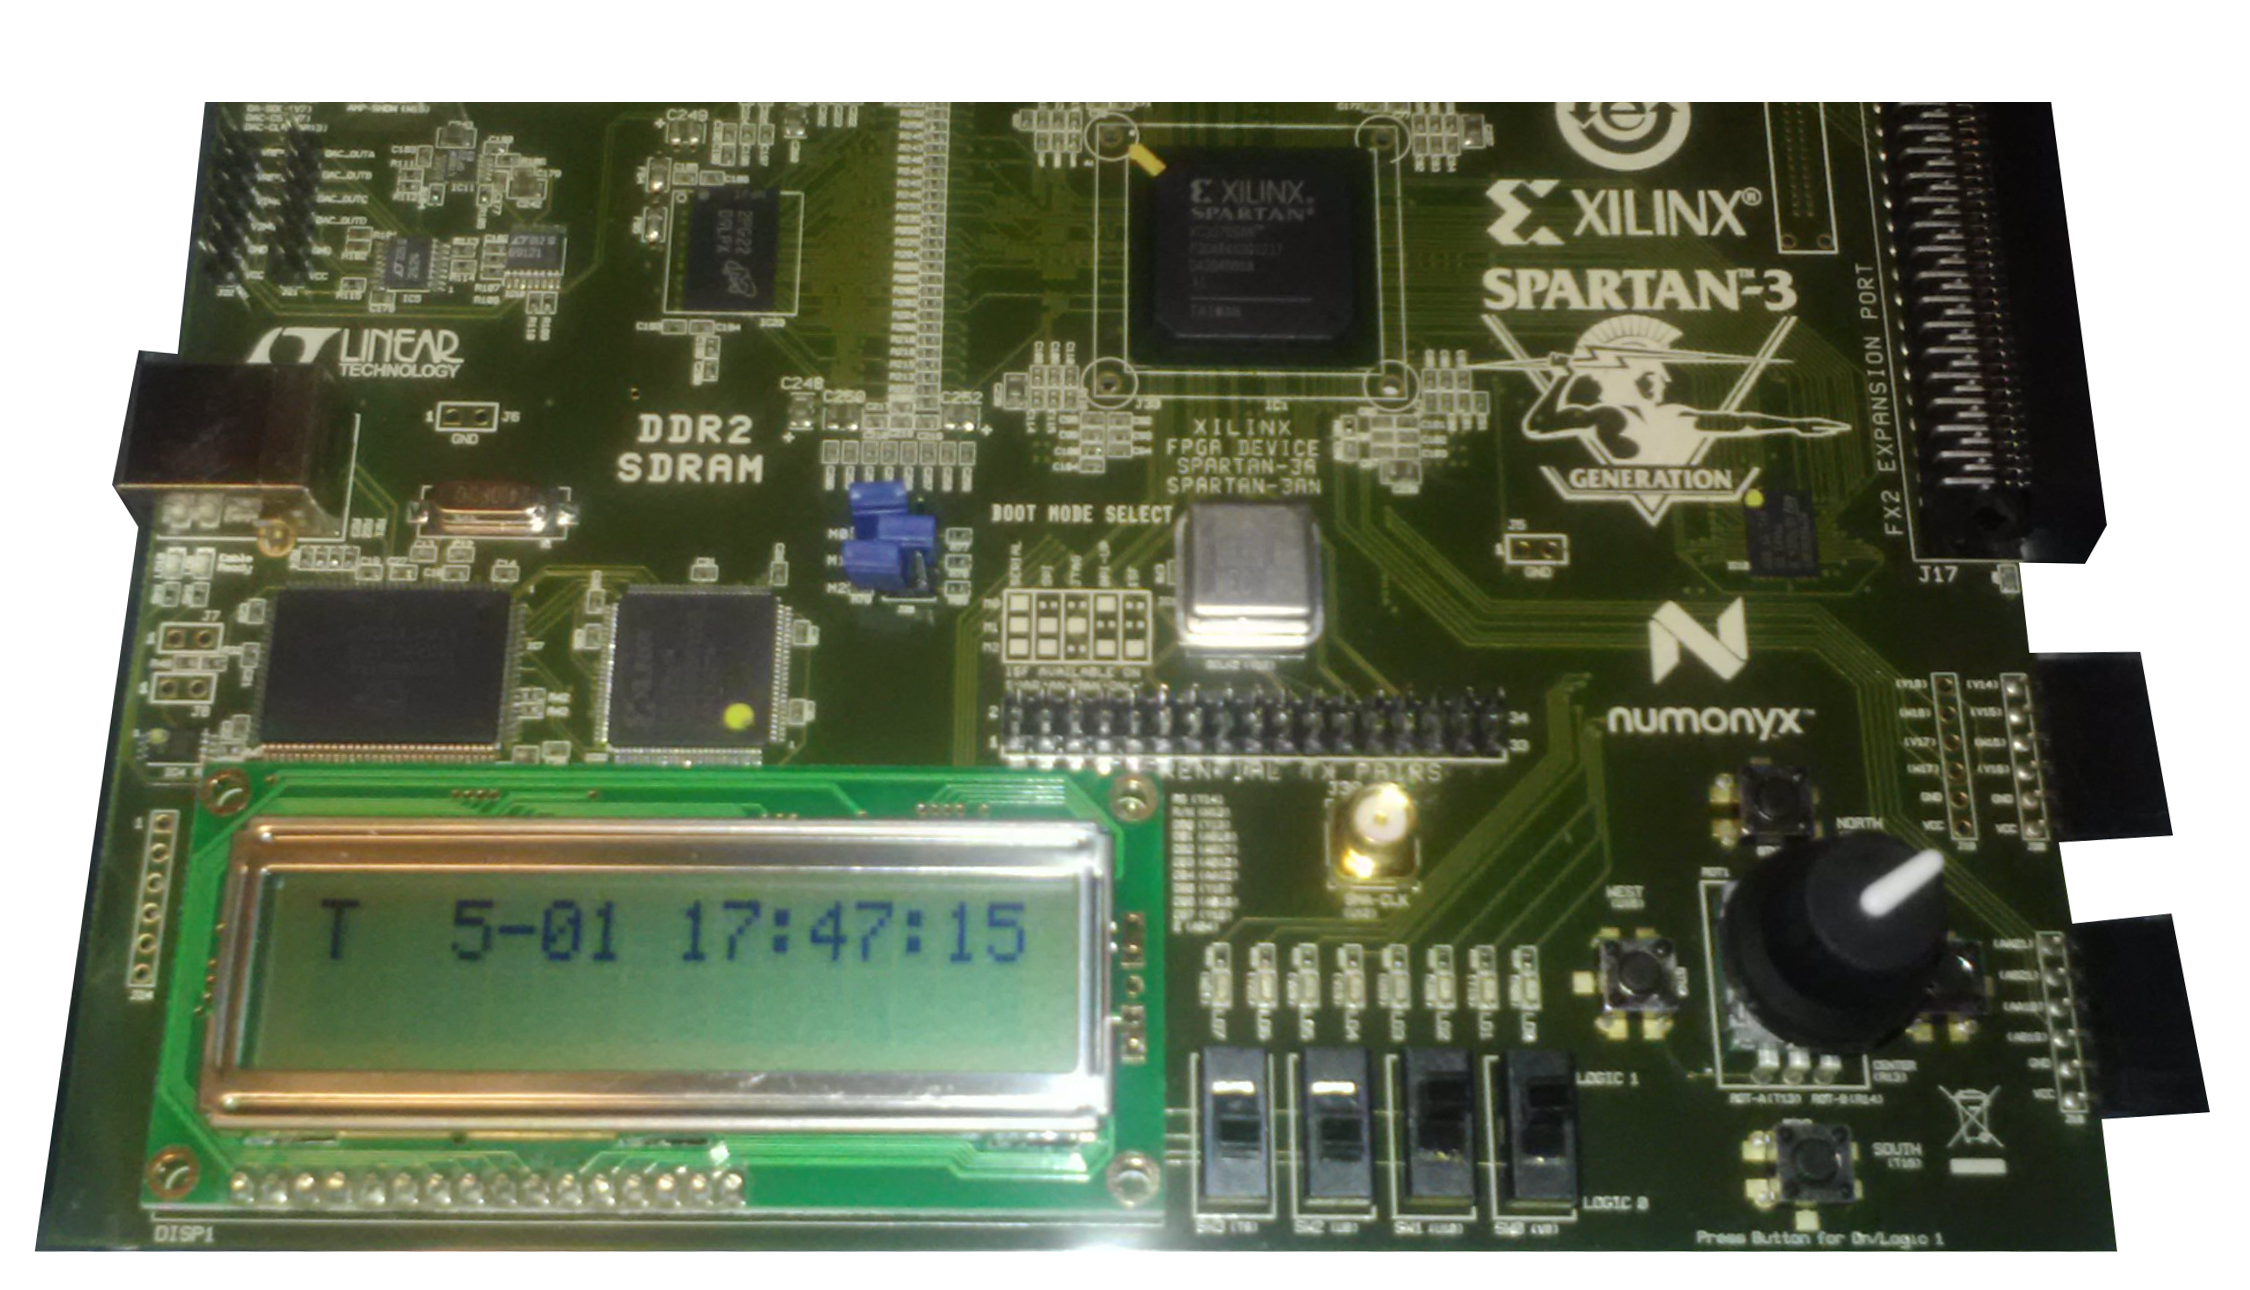
\includegraphics[width=0.7\linewidth]{Clock.png}
\label{fig:titleclock}
\end{figure}

\vspace{1em}

\HRule \\[0.4cm]
{ \huge \bfseries Real time clock final project\attachfile{main.tex}}\\[0.4cm] \footnote{Edward Maton checked my clock and it works exactly as described in this report:\attachfile{rtc.zip}} % Title of document
\HRule \\[1.5cm]

\begin{minipage}{0.4\textwidth}
\begin{flushleft} \large
\emph{Author:}\\
Seth \textsc{Miers} % Name
\end{flushleft}
\end{minipage}
~
\begin{minipage}{0.4\textwidth}
\begin{flushright} \large
\emph{Professor:} \\
Dr. Michael \textsc{Lightner}                                   % Professor's Name
\end{flushright}
\end{minipage}\\[4cm]

{\large May 1, 2013}\\[3cm]                                     % Date, change the \today to be precise

%\includegraphics{Logo}\\[1cm]                             % Include a department/university logo

\vspace*{\fill}                                            % Fill the rest of the page with whitespace

\end{titlepage}

\phantomsection

\tableofcontents                                           % These two lines are needed to
\addcontentsline{toc}{section}{Table of Contents}          % initialize and display TOC
\newpage

%----------------------------------------------------------------------------------------
%    CONTENT
%----------------------------------------------------------------------------------------

\section{Functionality}

\subsection{Reading the Display}

\begin{figure}[H]
\centering
\begin{tikzpicture}
    \node[anchor=south west,inner sep=0] at (0,0) {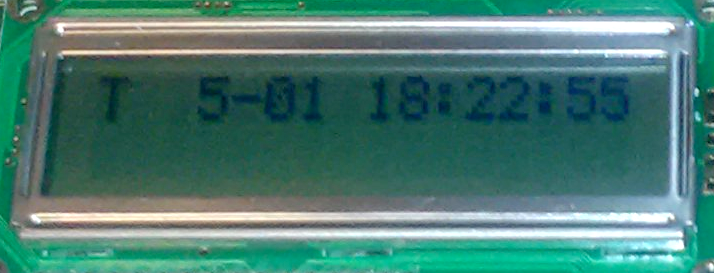
\includegraphics[width=0.5\textwidth]{display.png}};
    \draw[red,ultra thick,rounded corners] (0.9,1.6) rectangle (1.65,2.35);
    \draw[red,ultra thick] (1.375,1.6) -- (4,0.6);
    \node [red,below] at (4,0.6) {\Large Mode};
\end{tikzpicture}
\label{fig:modedisplay}
\end{figure}

The purpose of the single letter on the far left is to display which mode the clock is currently in. See \cref{sec:mode} to learn how to change between each of the 3 states: 

\begin{itemize}
  \item 'T' for 'time' - This displays the current time like any clock
  \item 'S' for 'set' - This is the value the time will set to when the set button is clicked
  \item 'A' for 'alarm' - This displays the time that the alarm will go off
\end{itemize}

\begin{figure}[H]
\centering
\begin{tikzpicture}
    \node[anchor=south west,inner sep=0] at (0,0) {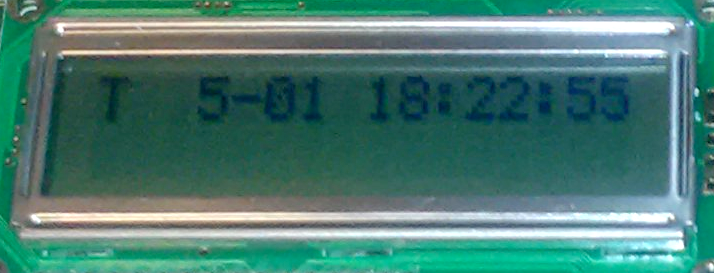
\includegraphics[width=0.5\textwidth]{display.png}};
    \draw[red,ultra thick,rounded corners] (1.9,1.6) rectangle (3.8,2.35);
    \draw[red,ultra thick] (2.85,1.6) -- (4,0.6);
    \node [red,below] at (4,0.6) {\Large Date};
\end{tikzpicture}
\label{fig:datedisplay}
\end{figure}

The date item displays the current month and day. Each month is programmed into the FPGA so you don't have to worry about how many days each month has. The date is in the format: (Month)-(Day).

\begin{figure}[H]
\centering
\begin{tikzpicture}
    \node[anchor=south west,inner sep=0] at (0,0) {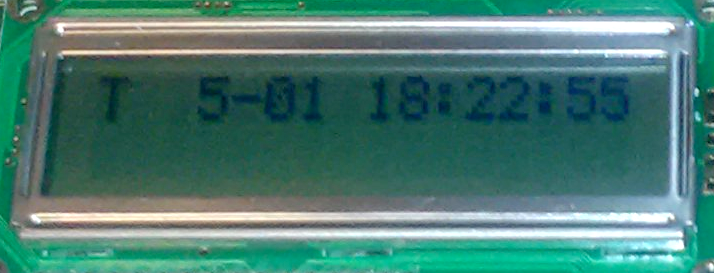
\includegraphics[width=0.5\textwidth]{display.png}};
    \draw[red,ultra thick,rounded corners] (3.8,1.6) rectangle (7.3,2.35);
    \draw[red,ultra thick] (5.55,1.6) -- (4,0.6);
    \node [red,below] at (4,0.6) {\Large Time};
\end{tikzpicture}
\label{fig:timedisplay}
\end{figure}

The time section displays the current time in a 24 hour format. The time is in the format: (hour):(minute):(second)

\subsection{Changing the mode}\label{sec:mode}

\begin{figure}[H]
\centering
\begin{tikzpicture}
    \node[anchor=south west,inner sep=0] at (0,0) {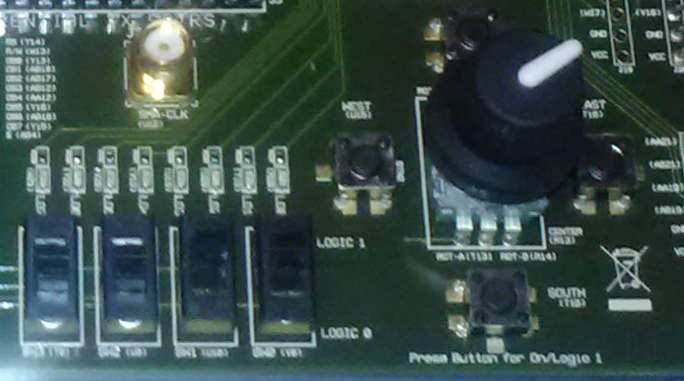
\includegraphics[width=0.5\textwidth]{buttons.png}};
    \draw[red,ultra thick,rounded corners] (4.8,1.6) rectangle (7.3,4.35);
    \draw[red,ultra thick] (6.05,1.6) -- (4,0.6);
    \node [red,below] at (4,0.6) {\Large Rotary Knob};
\end{tikzpicture}
\label{fig:changemode}
\end{figure}

The rotary knob can be clicked in. If you hold the rotary knob button down after \textonehalf \, of a second the mode will change in the order: $Time \to Set \to Alarm \to Time$ and repeats.

\subsection{Setting the time}

\begin{figure}[H]
\centering
\begin{tikzpicture}
    \node[anchor=south west,inner sep=0] at (0,0) {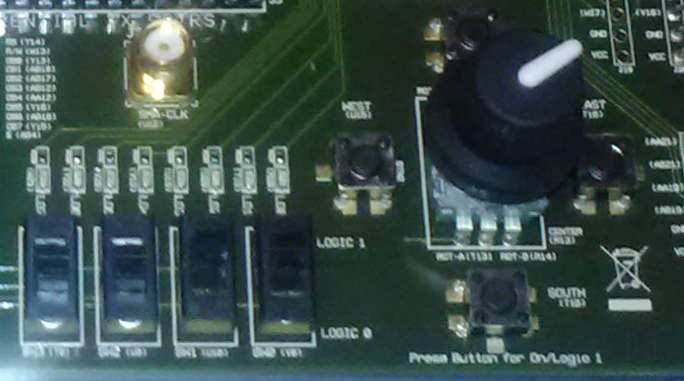
\includegraphics[width=0.5\textwidth]{buttons.png}};
    \draw[red,ultra thick,rounded corners] (5.4,0.6) rectangle (6.2,1.4);
    \draw[red,ultra thick] (5.8,0.6) -- (4,0.6);
    \node [red,below] at (4,0.6) {\Large Set Button};
\end{tikzpicture}
\label{fig:setbutton}
\end{figure}

The button just below the rotary knob is used to set the time. The time value in 'T' will store the time value in 'S' once the set button is pushed.

\subsection{Changing the set time and alarm time value}

To change the value you first need to know what you need to change. You can chage the seconds, the minutes, the hours, or the day. To change the month you have to increment through each day until the system rolls over, this is just due to the lack of switches on this particular FPGA board.

\begin{figure}[H]
\centering
\begin{tikzpicture}
    \node[anchor=south west,inner sep=0] at (0,0) {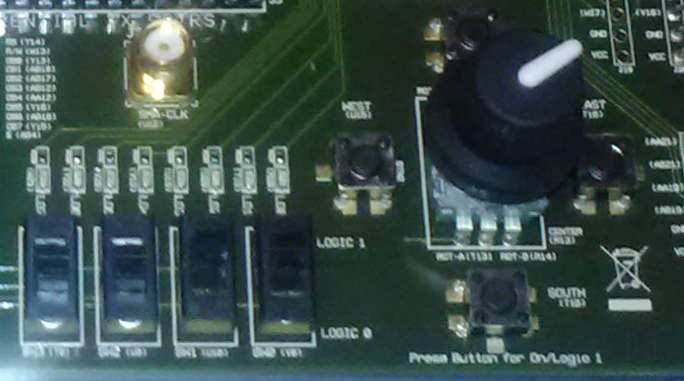
\includegraphics[width=0.5\textwidth]{buttons.png}};
    \draw[red,ultra thick,rounded corners] (1,0.6) rectangle (3.9,2.2);
    \draw[red,ultra thick] (2,0.6) -- (4,0.6);
    \node [red,below] at (4,0.6) {\Large Set Switches};
\end{tikzpicture}
\label{fig:setswitches}
\end{figure}

If all the switches are off then you will be able to set the seconds. If the right most switch is active (in the up position 001) then you will be able to set the minutes. If the middle switch is active (it doesn't matter what value the right most switch is 010 or 011) then you will be able to set the hours. Finally, if the left most switch is active, then you will be able to set the day.

\begin{figure}[H]
\centering
\begin{tikzpicture}
    \node[anchor=south west,inner sep=0] at (0,0) {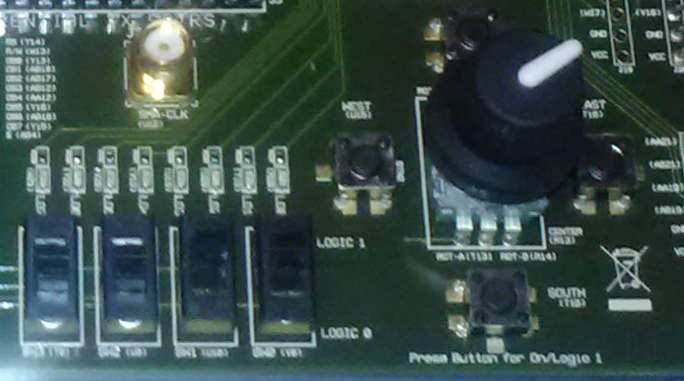
\includegraphics[width=0.5\textwidth]{buttons.png}};
    \draw[red,ultra thick,rounded corners] (4.8,1.6) rectangle (7.3,4.35);
    \draw[red,ultra thick] (6.05,1.6) -- (4,0.6);
    \node [red,below] at (4,0.6) {\Large Rotary Knob};
\end{tikzpicture}
\label{fig:incdecvalue}
\end{figure}

To change the value of the current thing you have selected (with the switches) you will need to rotate the rotary knob. Clockwise increments the value while counter-clockwise decrements the value.

\subsection{Turning on the alarm}

\begin{figure}[H]
\centering
\begin{tikzpicture}
    \node[anchor=south west,inner sep=0] at (0,0) {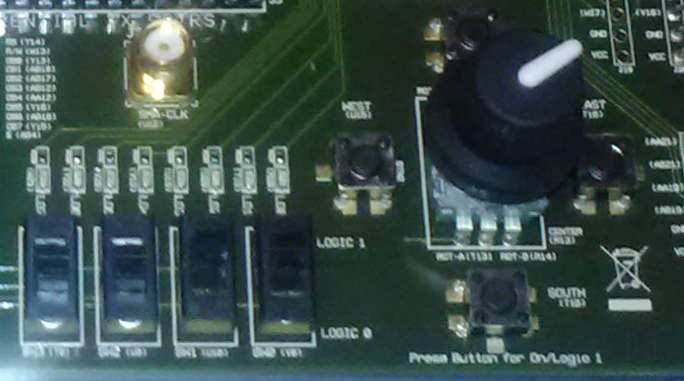
\includegraphics[width=0.5\textwidth]{buttons.png}};
    \draw[red,ultra thick,rounded corners] (0.1,0.6) rectangle (1,2.2);
    \draw[red,ultra thick] (0.2,0.6) -- (4,0.6);
    \node [red,below] at (4,0.6) {\Large Set Alarm};
\end{tikzpicture}
\label{fig:setalarm}
\end{figure}

The fourth most left switch is used to enable and disable the alarm. If the alarm is enabled the LED just above the switch will light up. As soon as the time value reaches the same minute as the alarm value, the rest of the LEDs above the switches will start flashing until the end of the minute or until the alarm is disabled via the switch.

\section{The code behind the 'GUI'}

\subsection{Clock module}

The clock module sets up a simple divider to take down the onboard 50MHz clock to 100Hz. The 100Hz is then used to drive most of the time values in the real time clock.

\begin{figure}[H]
\centering
\begin{lstlisting}[language=Verilog]
module Clock100(ClkIn,Clr_,Clk100);
  input ClkIn; // 50 MHz input
  input Clr_; // Clear all registers
  output reg Clk100; // Clock frequency

  reg [3:0] clk_div; // Set up a divider for the clock
  reg [13:0] clk_div100; // Set up the 100 Hz buffer counter

  always @(posedge ClkIn) // Pre-Scaler
  begin
    clk_div <= clk_div + 4'b1;
  end

  always @(posedge clk_div[3]) // Generate 100 Hz clock
  begin
    if (Clr_ == 1'b1 | clk_div100 == 14'b11110100001001)
      begin
        clk_div100 <= 14'b0;
        Clk100 <= ~Clk100; // Output clock signal
      end
    else
      clk_div100 <= clk_div100 + 19'b1; // Reset counter
  end

endmodule
\end{lstlisting}
\label{fig:clockmodule}
\end{figure}

The pre-scaler on line 11 is an initial divider to slim down the number of logic gates used in the entire circuit. Then at line 15, the actual divider starts to produce the 100Hz output.

\subsection{Spinner module}

The spinner module is specific to the Spartan-3AN FPGA. The way the signals are defined are in the Xilinx user guide for this FPGA.

\begin{figure}[H]
\centering
\begin{lstlisting}[language=Verilog]
`timescale 1 ns / 1 ps

module spinner
  (
  input  wire        sync_rot_a, // Left input defined on board
  input  wire        sync_rot_b, // Right input
  input  wire        clk, // 50MHz clock
  output reg         event_rot_l, // Output event
  output reg         event_rot_r  // Output event
  );

  reg                rotary_q1;
  reg                rotary_q2;
  reg                rotary_q1_dly;
  reg                rotary_q2_dly;

  always @(posedge clk)
  begin : filter
    case ({sync_rot_b, sync_rot_a}) // Look for change
      0: rotary_q1 <= 1'b0;
      1: rotary_q2 <= 1'b0;
      2: rotary_q2 <= 1'b1;
      3: rotary_q1 <= 1'b1;
    endcase
    rotary_q1_dly <= rotary_q1;
    rotary_q2_dly <= rotary_q2;
    event_rot_l <=  rotary_q2_dly && !rotary_q1_dly && rotary_q1;
    event_rot_r <= !rotary_q2_dly && !rotary_q1_dly && rotary_q1;
  end

endmodule
\end{lstlisting}
\label{fig:spinnermodule}
\end{figure}

Every time the knob is twisted it creates 2 clock edges for the direction it turned. Line 5 is the input wire for the left direction, and line 6 is the input for the right direction. This code just sets up a simple casestatement to check when the value of one of the directions have changed. When it changes it will output a pulse on the reg defined on line 8 and 9 for exactly 1 clock cycle. So for these signals to be read in somewhere else, they need to be read on the negative edge of the onboard 50MHz clock.

\subsection{LCD decoder module}

To make my life easier, instead of having to use the LCD codes in my clock, I designed an LCD decoder to convert from BCD to the LCD code.

\begin{lstlisting}[language=Verilog]
module lcd_decoder(
    input        clk,
     input        [1:0] set,
	 input        [2:0] m_seconds,
	 input        [3:0] l_seconds,
	 input        [2:0] m_minutes,
	 input        [3:0] l_minutes,
	 input        [1:0] m_hours,
	 input        [3:0] l_hours,
	 input        [1:0] m_days,
	 input        [3:0] l_days,
	 input              m_months,
	 input        [3:0] l_months,
	 output reg   [87:0] lcd_value
  );

  always @(posedge clk) begin
    case (l_seconds)
	   4'b0000: lcd_value[7:0] <= 8'b00110000;
		4'b0001: lcd_value[7:0] <= 8'b00110001;
		4'b0010: lcd_value[7:0] <= 8'b00110010;
		4'b0011: lcd_value[7:0] <= 8'b00110011;
		4'b0100: lcd_value[7:0] <= 8'b00110100;
		4'b0101: lcd_value[7:0] <= 8'b00110101;
		4'b0110: lcd_value[7:0] <= 8'b00110110;
		4'b0111: lcd_value[7:0] <= 8'b00110111;
		4'b1000: lcd_value[7:0] <= 8'b00111000;
		4'b1001: lcd_value[7:0] <= 8'b00111001;
		default: lcd_value[7:0] <= 8'b00110000;
	 endcase
    case (m_seconds)
	   3'b000: lcd_value[15:8] <= 8'b00110000;
		3'b001: lcd_value[15:8] <= 8'b00110001;
		3'b010: lcd_value[15:8] <= 8'b00110010;
		3'b011: lcd_value[15:8] <= 8'b00110011;
		3'b100: lcd_value[15:8] <= 8'b00110100;
		3'b101: lcd_value[15:8] <= 8'b00110101;
		default: lcd_value[15:8] <= 8'b00110000;
	 endcase
	 case (l_minutes)
	   4'b0000: lcd_value[23:16] <= 8'b00110000;
		4'b0001: lcd_value[23:16] <= 8'b00110001;
		4'b0010: lcd_value[23:16] <= 8'b00110010;
		4'b0011: lcd_value[23:16] <= 8'b00110011;
		4'b0100: lcd_value[23:16] <= 8'b00110100;
		4'b0101: lcd_value[23:16] <= 8'b00110101;
		4'b0110: lcd_value[23:16] <= 8'b00110110;
		4'b0111: lcd_value[23:16] <= 8'b00110111;
		4'b1000: lcd_value[23:16] <= 8'b00111000;
		4'b1001: lcd_value[23:16] <= 8'b00111001;
		default: lcd_value[23:16] <= 8'b00110000;
	 endcase
	 case (m_minutes)
	   3'b000: lcd_value[31:24] <= 8'b00110000;
		3'b001: lcd_value[31:24] <= 8'b00110001;
		3'b010: lcd_value[31:24] <= 8'b00110010;
		3'b011: lcd_value[31:24] <= 8'b00110011;
		3'b100: lcd_value[31:24] <= 8'b00110100;
		3'b101: lcd_value[31:24] <= 8'b00110101;
		default: lcd_value[31:24] <= 8'b00110000;
	 endcase
	 case (l_hours)
	   4'b0000: lcd_value[39:32] <= 8'b00110000;
		4'b0001: lcd_value[39:32] <= 8'b00110001;
		4'b0010: lcd_value[39:32] <= 8'b00110010;
		4'b0011: lcd_value[39:32] <= 8'b00110011;
		4'b0100: lcd_value[39:32] <= 8'b00110100;
		4'b0101: lcd_value[39:32] <= 8'b00110101;
		4'b0110: lcd_value[39:32] <= 8'b00110110;
		4'b0111: lcd_value[39:32] <= 8'b00110111;
		4'b1000: lcd_value[39:32] <= 8'b00111000;
		4'b1001: lcd_value[39:32] <= 8'b00111001;
		default: lcd_value[39:32] <= 8'b00110000;
	 endcase
	 case (m_hours)
	   2'b00: lcd_value[47:40] <= 8'b00100000;
		2'b01: lcd_value[47:40] <= 8'b00110001;
		2'b10: lcd_value[47:40] <= 8'b00110010;
		default: lcd_value[47:40] <= 8'b00100000;
	 endcase
	 case (l_days)
	   4'b0000: lcd_value[55:48] <= 8'b00110000;
		4'b0001: lcd_value[55:48] <= 8'b00110001;
		4'b0010: lcd_value[55:48] <= 8'b00110010;
		4'b0011: lcd_value[55:48] <= 8'b00110011;
		4'b0100: lcd_value[55:48] <= 8'b00110100;
		4'b0101: lcd_value[55:48] <= 8'b00110101;
		4'b0110: lcd_value[55:48] <= 8'b00110110;
		4'b0111: lcd_value[55:48] <= 8'b00110111;
		4'b1000: lcd_value[55:48] <= 8'b00111000;
		4'b1001: lcd_value[55:48] <= 8'b00111001;
		default: lcd_value[55:48] <= 8'b00110000;
	 endcase
	 case (m_days)
	   2'b00: lcd_value[63:56] <= 8'b00110000;
		2'b01: lcd_value[63:56] <= 8'b00110001;
		2'b10: lcd_value[63:56] <= 8'b00110010;
		2'b11: lcd_value[63:56] <= 8'b00110011;
		default: lcd_value[63:56] <= 8'b00110000;
	 endcase
	 case (l_months)
	   4'b0000: lcd_value[71:64] <= 8'b00110000;
		4'b0001: lcd_value[71:64] <= 8'b00110001;
		4'b0010: lcd_value[71:64] <= 8'b00110010;
		4'b0011: lcd_value[71:64] <= 8'b00110011;
		4'b0100: lcd_value[71:64] <= 8'b00110100;
		4'b0101: lcd_value[71:64] <= 8'b00110101;
		4'b0110: lcd_value[71:64] <= 8'b00110110;
		4'b0111: lcd_value[71:64] <= 8'b00110111;
		4'b1000: lcd_value[71:64] <= 8'b00111000;
		4'b1001: lcd_value[71:64] <= 8'b00111001;
		default: lcd_value[71:64] <= 8'b00110000;
	 endcase
	 case (m_months)
      1'b0: lcd_value[79:72] <= 8'b00100000;
		1'b1: lcd_value[79:72] <= 8'b00110001;
		default: lcd_value[79:72] <= 8'b00100000;
	 endcase
	 case (set)
	   2'b00: lcd_value[87:80] <= 8'b01010100;
		2'b01: lcd_value[87:80] <= 8'b01010011;
		2'b10: lcd_value[87:80] <= 8'b01000001;
		default: lcd_value[87:80] <= 8'b00100000;
	 endcase
  end


endmodule
\end{lstlisting}

Without diving in deep into the exact code specifications for how the LCD screen operates, it's tricky to explain exactly how this code works. However, it opperates in roughly the same manner as a 7-segment display decoder would. It takes a BCD value for several different inputs and converts it to a coded value for the LCD screen.

\subsection{LCD display module}

The LCD display module is, once again, just a bunch of values required by the microcontroller on the Spartan-3AN. 

\begin{lstlisting}[language=Verilog]
// synthesis attribute STEPPING top "ES"
module lcd_display (clk, value, lcd_rs, lcd_rw, lcd_e, lcd_4, lcd_5, lcd_6, lcd_7);
parameter       n = 26;
parameter       k = 17;
input           clk;
input           [87:0] value;
reg             [n-1:0] count = 0;
reg             lcd_busy = 1'b1;
reg             lcd_stb;
reg             [5:0] lcd_code = 6'b000000;
//reg             [87:0] value = 88'b0010000000100000001000000010000000
100000001000000010000000100000001000000010000000100000;
output reg      lcd_rs;
output reg      lcd_rw;
output reg      lcd_7;
output reg      lcd_6;
output reg      lcd_5;
output reg      lcd_4;
output reg      lcd_e;


  always @ (posedge clk) begin
    count <= count + 1;
    case (count[k+8:k+2])
       0: lcd_code <= 6'b000010;           // function set
       1: lcd_code <= 6'b000010;
       2: lcd_code <= 6'b001100;
       3: lcd_code <= 6'b000000;           // display on/off control
       4: lcd_code <= 6'b001100;
       5: lcd_code <= 6'b000000;           // display clear
       6: lcd_code <= 6'b000001;
       7: lcd_code <= 6'b000000;           // entry mode set
       8: lcd_code <= 6'b000110;
       9: lcd_code <= 6'b000000;           //clear display
	  10: lcd_code <= 6'b000001;
      11: lcd_code <= 6'b001000;           //cursor position
      12: lcd_code <= 6'b000000;
      13: lcd_code <= {2'b10,value[87:84]};// 1 Set or Space
      14: lcd_code <= {2'b10,value[83:80]};
      15: lcd_code <= 6'b100010;           // 2 Space
      16: lcd_code <= 6'b100000;
      17: lcd_code <= {2'b10,value[79:76]};// 3 most month
      18: lcd_code <= {2'b10,value[75:72]};
      19: lcd_code <= {2'b10,value[71:68]};// 4 least month
      20: lcd_code <= {2'b10,value[67:64]};
	  21: lcd_code <= 6'b100010; // 5 hyphen
      22: lcd_code <= 6'b101101;
      23: lcd_code <= {2'b10,value[63:60]};// 6 most day
      24: lcd_code <= {2'b10,value[59:56]};
      25: lcd_code <= {2'b10,value[55:52]};// 7 least day
      26: lcd_code <= {2'b10,value[51:48]};
      27: lcd_code <= 6'b100010;           // 8 space
      28: lcd_code <= 6'b100000;
	  29: lcd_code <= {2'b10,value[47:44]};// 9 most hour
      30: lcd_code <= {2'b10,value[43:40]};
      31: lcd_code <= {2'b10,value[39:36]};// 10 least hour
      32: lcd_code <= {2'b10,value[35:32]};
      33: lcd_code <= 6'b100011;           // l1 collon
      34: lcd_code <= 6'b101010;
      35: lcd_code <= {2'b10,value[31:28]};// 12 most minute
      36: lcd_code <= {2'b10,value[27:24]};
	  37: lcd_code <= {2'b10,value[23:20]};// 13 least minute
      38: lcd_code <= {2'b10,value[19:16]};
      39: lcd_code <= 6'b100011;           // 14 collon
      40: lcd_code <= 6'b101010;
      41: lcd_code <= {2'b10,value[15:12]};// 15 most second
      42: lcd_code <= {2'b10,value[11:8]};
      43: lcd_code <= {2'b10,value[7:4]};  // 16 least second
      44: lcd_code <= {2'b10,value[3:0]};
	  45: count[k+8:k+2] <= 7'b0001011;
      default: begin
		  count[k+8:k+2] <= 7'b0001011;
		  //value <= lcd_value;
		end
    endcase
    if (lcd_rw)
      lcd_busy <= 0;
    lcd_stb <= ^count[k+1:k+0] & ~lcd_rw & lcd_busy;  // clkrate / 2^(k+2)
    {lcd_e,lcd_rs,lcd_rw,lcd_7,lcd_6,lcd_5,lcd_4} <= {lcd_stb,lcd_code};
  end
endmodule
\end{lstlisting}

The code is commented to help make understanding what the LCD coded values do a little bit easier. To display a character 2 different lines need to be sent to the microcontroller on the LCD screen. I set some of the characters constant, like for the collons or hyphen.

\subsection{Pin constraints}

Since the clock code is so long and in-depth, I decided to show the pin constraints first. 

\begin{lstlisting}[language=Verilog]
NET "clk" LOC = "E12";
NET "reset" LOC = "T15" | IOSTANDARD = LVCMOS33;

NET "minute_set" LOC = "V8" | IOSTANDARD = LVCMOS33;
NET "hour_set" LOC = "U10" | IOSTANDARD = LVCMOS33;
NET "day_set" LOC = "U8" | IOSTANDARD = LVCMOS33;
NET "alarm_set" LOC = "T9" | IOSTANDARD = LVCMOS33;

NET "ROT_A" LOC = "T13" | IOSTANDARD = LVCMOS33 | PULLUP ;
NET "ROT_B" LOC = "R14" | IOSTANDARD = LVCMOS33 | PULLUP ;
NET "ROT_CENTER" LOC = "R13" | IOSTANDARD = LVCMOS33 | PULLDOWN | CLOCK_DEDICATED_ROUTE = FALSE;

NET "alarm_on" LOC = "W21" | IOSTANDARD = LVCMOS33;
NET "alarm_led[0]" LOC = "V20" | IOSTANDARD = LVCMOS33;
NET "alarm_led[1]" LOC = "V19" | IOSTANDARD = LVCMOS33;
NET "alarm_led[2]" LOC = "U19" | IOSTANDARD = LVCMOS33;
NET "alarm_led[3]" LOC = "R20" | IOSTANDARD = LVCMOS33;
NET "alarm_led[4]" LOC = "T19" | IOSTANDARD = LVCMOS33;
NET "alarm_led[5]" LOC = "U20" | IOSTANDARD = LVCMOS33;

NET "lcd_e" LOC = "AB4" | IOSTANDARD = LVCMOS33 | DRIVE = 4 | SLEW = SLOW ;
NET "lcd_rs" LOC = "Y14" | IOSTANDARD = LVCMOS33 | DRIVE = 4 | SLEW = SLOW ;
NET "lcd_rw" LOC = "W13" | IOSTANDARD = LVCMOS33 | DRIVE = 4 | SLEW = SLOW ;
NET "lcd_7" LOC = "Y15" | IOSTANDARD = LVCMOS33 | DRIVE = 4 | SLEW = SLOW ;
NET "lcd_6" LOC = "AB16" | IOSTANDARD = LVCMOS33 | DRIVE = 4 | SLEW = SLOW ;
NET "lcd_5" LOC = "Y16" | IOSTANDARD = LVCMOS33 | DRIVE = 4 | SLEW = SLOW ;
NET "lcd_4" LOC = "AA12" | IOSTANDARD = LVCMOS33 | DRIVE = 4 | SLEW = SLOW ;
\end{lstlisting}

Some of the pins on the Spartan-3AN need to be attached to a pull-up resistor when being used as a user input. Adding a pullup also helps a little bit with debouncing the button, even though a debouncing capacitor is already implemented in this particular FPGA.

\subsection{Real time clock module}

Due to the nature of this code and how it handles days as well as several different settings, it is very large, so I will split it into sub sections to explain it.

\subsubsection{The header}

\begin{lstlisting}[language=Verilog]
module rtc(
    input ROT_A,
    input ROT_B,
    input ROT_CENTER,
    input minute_set,
    input hour_set,
    input day_set,
    input alarm_set,
    input clk,
     input reset,
	 output reg alarm_on,
	 output reg [5:0] alarm_led,
    output lcd_rs,
    output lcd_rw,
    output lcd_7,
    output lcd_6,
    output lcd_5,
    output lcd_4,
    output lcd_e
  );

  wire [87:0] lcd_value;
  wire hundred_clk;
  
  wire event_rot_l;
  wire event_rot_r;
  
  reg second_clk;
  reg minute_clk;
  reg hour_clk;
  reg day_clk;
  reg [1:0] mode = 2'b00;
  reg [5:0] sec_count = 6'b000000;
  reg alarm_start = 1'b0;
  reg [6:0] alarm_count = 7'b0000000;
  
  reg        [2:0] m_seconds = 3'b000;  // Section where the current Time regs are
  reg        [3:0] l_seconds = 4'b0000;
  reg        [2:0] m_minutes = 3'b000;
  reg        [3:0] l_minutes = 4'b0000;
  reg        [1:0] m_hours = 2'b00;
  reg        [3:0] l_hours = 4'b0000;
  reg        [1:0] m_days = 2'b00;
  reg        [3:0] l_days = 4'b0001;
  reg        [3:0] months = 4'b0001;
  
  reg        [2:0] sm_seconds = 3'b000;  // Section where the current Set regs are
  reg        [3:0] sl_seconds = 4'b0000;
  reg        [2:0] sm_minutes = 3'b000;
  reg        [3:0] sl_minutes = 4'b0000;
  reg        [1:0] sm_hours = 2'b00;
  reg        [3:0] sl_hours = 4'b0000;
  reg        [1:0] sm_days = 2'b00;
  reg        [3:0] sl_days = 4'b0001;
  reg        [3:0] smonths = 4'b0001;
  
  reg        [2:0] am_seconds = 3'b000;  // Section where the current Alarm regs are
  reg        [3:0] al_seconds = 4'b0000;
  reg        [2:0] am_minutes = 3'b000;
  reg        [3:0] al_minutes = 4'b0000;
  reg        [1:0] am_hours = 2'b00;
  reg        [3:0] al_hours = 4'b0000;
  reg        [1:0] am_days = 2'b00;
  reg        [3:0] al_days = 4'b0001;
  reg        [3:0] amonths = 4'b0001;
  
  reg        [2:0] cm_seconds = 3'b000;
  reg        [3:0] cl_seconds = 4'b0000;
  reg        [2:0] cm_minutes = 3'b000;
  reg        [3:0] cl_minutes = 4'b0000;
  reg        [1:0] cm_hours = 2'b00;
  reg        [3:0] cl_hours = 4'b0000;
  reg        [1:0] cm_days = 2'b00;
  reg        [3:0] cl_days = 4'b0001;
  reg              cm_months = 1'b0;
  reg        [3:0] cl_months = 4'b0001;
\end{lstlisting}

The first section of code sets up every single input and output I will need to create a fully functional real time clock. The outputs and inputs were described at the begining of this document. The reg values are used to define how often a second, minute, hour, or day should increment, what mode the clock is in, or transition lines from the time value, set value, or alarm value to the display.

\subsubsection{Spinner and clock}

\begin{lstlisting}[language=Verilog,firstnumber=78]
  spinner knob(ROT_A,ROT_B,clk,event_rot_l,event_rot_r);
  
  always @(posedge second_clk) begin
    if (ROT_CENTER) begin
      mode <= mode + 1;
      if (mode == 2'b10)
         mode <= mode + 2;
    end
  end

  Clock100 timer(clk,reset,hundred_clk);
  
  always @(posedge hundred_clk or posedge reset) begin
    if (reset) begin
	   sec_count <= 6'b000000;
	 end else begin
      if (reset | sec_count == 6'b110001) begin
	     sec_count <= 6'b000000;
		  second_clk <= ~second_clk;
  	   end
	   else
	     sec_count <= sec_count + 1;
	 end
  end
\end{lstlisting}

The spinner module is simple attached at the begining to the clock event lines so that they can be read in by other always blocks. On line 80 I used the positive edge of the second timer to activate the mode change, this mode change is only activated if the center button on the rotary knob is pshed down. I learned that the center button on the rotary knob is not debounced like the rest of the buttons, so implementing this also prevents false signals.\\
Finally the clock 100Hz timer is tied to an always blocks that counts up until it reaches 50, then it changes the value of the second clock. This yeils a 1Hz signal on the second_clk line.

\subsubsection{Normal Clock}

\begin{lstlisting}[language=Verilog,firstnumber=103]
  always @ (posedge second_clk or posedge reset)
  begin
    l_seconds <= l_seconds + 1;
     minute_clk <= 1'b0;
	 if (reset) begin
	   l_seconds <= sl_seconds;
		m_seconds <= sm_seconds;
	 end else begin
	   if (l_seconds == 4'b1001 && m_seconds == 3'b101) begin
	     l_seconds <= 4'b0000;
	  	  m_seconds <= 3'b000;
		  minute_clk <= 1'b1;
	   end else if (l_seconds == 4'b1001) begin
		  l_seconds <= 4'b0000;
		  m_seconds <= m_seconds + 1;
	   end
	 end
  end
  

  always @ (posedge minute_clk or posedge reset)
  begin
    l_minutes <= l_minutes + 1;
	 hour_clk <= 1'b0;
	 if (reset) begin
	   l_minutes <= sl_minutes;
		m_minutes <= sm_minutes;
	 end else begin
	   if (l_minutes == 4'b1001 && m_minutes == 3'b101) begin
	     l_minutes <= 4'b0000;
	  	  m_minutes <= 3'b000;
		  hour_clk <= 1'b1;
	   end else if (l_minutes == 4'b1001) begin
		  l_minutes <= 4'b0000;
		  m_minutes <= m_minutes + 1;
	   end
	 end
  end
  
 
  always @ (posedge hour_clk or posedge reset)
  begin
    l_hours <= l_hours + 1;
	 day_clk <= 1'b0;
	 if (reset) begin
	   l_hours <= sl_hours;
		m_hours <= sm_hours;
	 end else begin
	   if (l_hours == 4'b0011 && m_hours == 3'b010) begin
	     l_hours <= 4'b0000;
	  	  m_hours <= 3'b000;
		  day_clk <= 1'b1;
	   end else if (l_hours == 4'b1001) begin
		  l_hours <= 4'b0000;
		  m_hours <= m_hours + 1;
	   end
	 end
  end
  
  always @ (posedge day_clk or posedge reset)
  begin
    l_days <= l_days + 4'b1;
	 if (reset) begin
	   l_days <= sl_days;
		m_days <= sm_days;
		months <= smonths;
	 end else begin
      case (months)
		  1,3,5,7,8,10: begin
	         if (l_days == 4'b0001 && m_days == 2'b11) begin
	           l_days <= 4'b0001;
	        	  m_days <= 2'b00;
				  months <= months + 1;
	         end else if (l_days == 4'b1010) begin
		        l_days <= 4'b0000;
		        m_days <= m_days + 1;
	         end
		    end
		  4,6,9,11: begin
	         if (m_days == 2'b11) begin
	           l_days <= 4'b0001;
	        	  m_days <= 2'b00;
				  months <= months + 1;
	         end else if (l_days == 4'b1010) begin
		        l_days <= 4'b0000;
		        m_days <= m_days + 1;
	         end
		    end
		  2: begin
	         if (l_days == 4'b1000 && m_days == 2'b10) begin
	           l_days <= 4'b0001;
	        	  m_days <= 2'b00;
				  months <= months + 1;
	         end else if (l_days == 4'b1010) begin
		        l_days <= 4'b0000;
		        m_days <= m_days + 1;
	         end
		    end
		  12: begin
	         if (l_days == 4'b0001 && m_days == 2'b11) begin
	           l_days <= 4'b0001;
	        	  m_days <= 2'b00;
				  months <= 4'b0001;
	         end else if (l_days == 4'b1010) begin
		        l_days <= 4'b0000;
		        m_days <= m_days + 1;
	         end
		    end
		endcase
	 end
  end
\end{lstlisting}

The block of code used for the normal clock is what ends up being shown as Time on the LCD display. There are several always blocks that are always looking for a pulse on the respective day, hour, minute, or second clock. However, there is also a reset value, which is what ends up setting the time to the set value.\\
The only tricky part about this code is the case statement for the months. I had to know exactly at what day for each month that the clock should roll over, and I had to design the state machine accordingly.

\subsubsection{Set clock}

\begin{lstlisting}[language=Verilog,firstnumber=216]
// Set Clock
  always @ (negedge clk)
  begin
    if (mode == 2'b01) begin
    case ({day_set,hour_set,minute_set})
       3'b000: begin
		    if (event_rot_l) begin
			   sl_seconds <= sl_seconds + 1;
 			   if (sl_seconds == 4'b1001 && sm_seconds == 3'b101) begin
			     sl_seconds <= 4'b0000;
			     sm_seconds <= 3'b000;
			   end else if (sl_seconds == 4'b1001) begin
			     sl_seconds <= 4'b0000;
			     sm_seconds <= sm_seconds + 1;
			   end
		    end else if (event_rot_r) begin
				    sl_seconds <= sl_seconds - 1;
			   if (sl_seconds == 4'b0000 && sm_seconds == 3'b000) begin
			     sl_seconds <= 4'b1001;
			     sm_seconds <= 3'b101;
			   end else if (sl_seconds == 4'b0000) begin
			     sl_seconds <= 4'b1001;
			     sm_seconds <= sm_seconds - 1;
			   end
		    end
	     end
	   3'b001: begin
		    if (event_rot_l) begin
			   sl_minutes <= sl_minutes + 1;
 			   if (sl_minutes == 4'b1001 && sm_minutes == 3'b101) begin
			     sl_minutes <= 4'b0000;
			     sm_minutes <= 3'b000;
			   end else if (sl_minutes == 4'b1001) begin
			     sl_minutes <= 4'b0000;
			     sm_minutes <= sm_minutes + 1;
			   end
		    end else if (event_rot_r) begin
				    sl_minutes <= sl_minutes - 1;
			   if (sl_minutes == 4'b0000 && sm_minutes == 3'b000) begin
			     sl_minutes <= 4'b1001;
			     sm_minutes <= 3'b101;
			   end else if (sl_minutes == 4'b0000) begin
			     sl_minutes <= 4'b1001;
			     sm_minutes <= sm_minutes - 1;
			   end
		    end
		  end
		3'b010,3'b011: begin
		    if (event_rot_l) begin
			   sl_hours <= sl_hours + 1;
 			   if (sl_hours == 4'b0011 && sm_hours == 2'b10) begin
			     sl_hours <= 4'b0000;
			     sm_hours <= 2'b00;
			   end else if (sl_hours == 4'b1001) begin
			     sl_hours <= 4'b0000;
			     sm_hours <= sm_hours + 1;
			   end
		    end else if (event_rot_r) begin
				    sl_hours <= sl_hours - 1;
			   if (sl_hours == 4'b0000 && sm_hours == 2'b00) begin
			     sl_hours <= 4'b0011;
			     sm_hours <= 2'b10;
			   end else if (sl_hours == 4'b0000) begin
			     sl_hours <= 4'b1001;
			     sm_hours <= sm_hours - 1;
			   end
		    end
		  end
		3'b100,3'b101,3'b110,3'b111: begin
		    if (event_rot_l) begin
			 sl_days <= sl_days + 4'b1;
			 case (smonths)
			   1,3,5,7,8,10: begin
				 	 if (sl_days == 4'b0001 && sm_days == 2'b11) begin
					   sl_days <= 4'b0001;
					   sm_days <= 2'b00;
					   smonths <= smonths + 1;
					 end else if (sl_days == 4'b1001) begin
					   sl_days <= 4'b0000;
					   sm_days <= sm_days + 1;
					 end
				  end
			   4,6,9,11: begin
					 if (sm_days == 2'b11) begin
					   sl_days <= 4'b0001;
					   sm_days <= 2'b00;
					   smonths <= smonths + 1;
					 end else if (sl_days == 4'b1001) begin
					   sl_days <= 4'b0000;
					   sm_days <= sm_days + 1;
					 end
				  end
			   2: begin
					 if (sl_days == 4'b1000 && sm_days == 2'b10) begin
					   sl_days <= 4'b0001;
					   sm_days <= 2'b00;
					   smonths <= smonths + 1;
					 end else if (sl_days == 4'b1001) begin
					   sl_days <= 4'b0000;
					   sm_days <= sm_days + 1;
					 end
				  end
			   12: begin
					 if (sl_days == 4'b0001 && sm_days == 2'b11) begin
					   sl_days <= 4'b0001;
					   sm_days <= 2'b00;
					   smonths <= 4'b0001;
					 end else if (sl_days == 4'b1001) begin
					   sl_days <= 4'b0000;
					   sm_days <= sm_days + 1;
					 end
				  end
			 endcase
		    end
		    if (event_rot_r) begin
			 sl_days <= sl_days - 4'b1;
			 case (smonths)
			   2,4,6,8,9,11: begin
				 	 if (sl_days == 4'b0001 && sm_days == 2'b00) begin
					   sl_days <= 4'b0001;
					   sm_days <= 2'b11;
					   smonths <= smonths - 1;
					 end else if (sl_days == 4'b0000) begin
					   sl_days <= 4'b1001;
					   sm_days <= sm_days - 1;
					 end
				  end
			   5,7,10,12: begin
					 if (sm_days == 2'b00 && sl_days == 4'b0001) begin
					   sl_days <= 4'b0001;
					   sm_days <= 2'b11;
					   smonths <= smonths - 1;
					 end else if (sl_days == 4'b0000) begin
					   sl_days <= 4'b1001;
					   sm_days <= sm_days - 1;
					 end
				  end
			   3: begin
					 if (sl_days == 4'b0001 && sm_days == 2'b00) begin
					   sl_days <= 4'b1000;
					   sm_days <= 2'b10;
					   smonths <= smonths - 1;
					 end else if (sl_days == 4'b0000) begin
					   sl_days <= 4'b1001;
					   sm_days <= sm_days - 1;
					 end
				  end
			   1: begin
					 if (sl_days == 4'b0001 && sm_days == 2'b00) begin
					   sl_days <= 4'b0001;
					   sm_days <= 2'b11;
					   smonths <= 4'b1100;
					 end else if (sl_days == 4'b0000) begin
					   sl_days <= 4'b1001;
					   sm_days <= sm_days - 1;
					 end
				  end
			 endcase
		    end
		  end
	 endcase
	 end
  end
\end{lstlisting}

The 'Set clock' section only differs slightly from the time section. Since setting the value does not need to rely upon any type of internal clock, I changed the code to depend on the left and right turn signals of the rotary knob. It checks for these events on the negative edge of the internal 50MHz clock so that these events will be catched properly. There is also a case statement implemented so that the FPGA knows which value it should increment or decrement (days, hours, minutes, or seconds). Finally, the only thing that really differs from the previous section is that there are 2 different case statements for the months. Since months don't roll over uniformly, a different state machine has to be designed depending on which direction the knob is turning. For all the maching knows you could be going from a 28 day month to a 31 day month, or from a 30 day month to a 31 day month. Having a second state machine prevents the FPGA from getting into an unknown state.

\subsubsection{Alarm clock}

\begin{lstlisting}[language=Verilog,firstnumber=380]
// Set Alarm
  always @ (negedge clk)
  begin
    if (mode == 2'b10) begin
    case ({day_set,hour_set,minute_set})
       3'b000: begin
		    if (event_rot_l) begin
			   al_seconds <= al_seconds + 1;
 			   if (al_seconds == 4'b1001 && am_seconds == 3'b101) begin
			     al_seconds <= 4'b0000;
			     am_seconds <= 3'b000;
			   end else if (al_seconds == 4'b1001) begin
			     al_seconds <= 4'b0000;
			     am_seconds <= am_seconds + 1;
			   end
		    end else if (event_rot_r) begin
				    al_seconds <= al_seconds - 1;
			   if (al_seconds == 4'b0000 && am_seconds == 3'b000) begin
			     al_seconds <= 4'b1001;
			     am_seconds <= 3'b101;
			   end else if (al_seconds == 4'b0000) begin
			     al_seconds <= 4'b1001;
			     am_seconds <= am_seconds - 1;
			   end
		    end
	     end
	   3'b001: begin
		    if (event_rot_l) begin
			   al_minutes <= al_minutes + 1;
 			   if (al_minutes == 4'b1001 && am_minutes == 3'b101) begin
			     al_minutes <= 4'b0000;
			     am_minutes <= 3'b000;
			   end else if (al_minutes == 4'b1001) begin
			     al_minutes <= 4'b0000;
			     am_minutes <= am_minutes + 1;
			   end
		    end else if (event_rot_r) begin
				    al_minutes <= al_minutes - 1;
			   if (al_minutes == 4'b0000 && am_minutes == 3'b000) begin
			     al_minutes <= 4'b1001;
			     am_minutes <= 3'b101;
			   end else if (al_minutes == 4'b0000) begin
			     al_minutes <= 4'b1001;
			     am_minutes <= am_minutes - 1;
			   end
		    end
		  end
		3'b010,3'b011: begin
		    if (event_rot_l) begin
			   al_hours <= al_hours + 1;
 			   if (al_hours == 4'b0011 && am_hours == 2'b10) begin
			     al_hours <= 4'b0000;
			     am_hours <= 2'b00;
			   end else if (al_hours == 4'b1001) begin
			     al_hours <= 4'b0000;
			     am_hours <= am_hours + 1;
			   end
		    end else if (event_rot_r) begin
				    al_hours <= al_hours - 1;
			   if (al_hours == 4'b0000 && am_hours == 2'b00) begin
			     al_hours <= 4'b0011;
			     am_hours <= 2'b10;
			   end else if (al_hours == 4'b0000) begin
			     al_hours <= 4'b1001;
			     am_hours <= am_hours - 1;
			   end
		    end
		  end
		3'b100,3'b101,3'b110,3'b111: begin
		    if (event_rot_l) begin
			 al_days <= al_days + 4'b1;
			 case (amonths)
			   1,3,5,7,8,10: begin
				 	 if (al_days == 4'b0001 && am_days == 2'b11) begin
					   al_days <= 4'b0001;
					   am_days <= 2'b00;
					   amonths <= amonths + 1;
					 end else if (al_days == 4'b1001) begin
					   al_days <= 4'b0000;
					   am_days <= am_days + 1;
					 end
				  end
			   4,6,9,11: begin
					 if (am_days == 2'b11) begin
					   al_days <= 4'b0001;
					   am_days <= 2'b00;
					   amonths <= amonths + 1;
					 end else if (al_days == 4'b1001) begin
					   al_days <= 4'b0000;
					   am_days <= am_days + 1;
					 end
				  end
			   2: begin
					 if (al_days == 4'b1000 && am_days == 2'b10) begin
					   al_days <= 4'b0001;
					   am_days <= 2'b00;
					   amonths <= amonths + 1;
					 end else if (al_days == 4'b1001) begin
					   al_days <= 4'b0000;
					   am_days <= am_days + 1;
					 end
				  end
			   12: begin
					 if (al_days == 4'b0001 && am_days == 2'b11) begin
					   al_days <= 4'b0001;
					   am_days <= 2'b00;
					   amonths <= 4'b0001;
					 end else if (al_days == 4'b1001) begin
					   al_days <= 4'b0000;
					   am_days <= am_days + 1;
					 end
				  end
			 endcase
		    end
		    if (event_rot_r) begin
			 al_days <= al_days - 4'b1;
			 case (amonths)
			   2,4,6,8,9,11: begin
				 	 if (al_days == 4'b0001 && am_days == 2'b00) begin
					   al_days <= 4'b0001;
					   am_days <= 2'b11;
					   amonths <= amonths - 1;
					 end else if (al_days == 4'b0000) begin
					   al_days <= 4'b1001;
					   am_days <= am_days - 1;
					 end
				  end
			   5,7,10,12: begin
					 if (am_days == 2'b00 && al_days == 4'b0001) begin
					   al_days <= 4'b0001;
					   am_days <= 2'b11;
					   amonths <= amonths - 1;
					 end else if (al_days == 4'b0000) begin
					   al_days <= 4'b1001;
					   am_days <= am_days - 1;
					 end
				  end
			   3: begin
					 if (al_days == 4'b0001 && am_days == 2'b00) begin
					   al_days <= 4'b1000;
					   am_days <= 2'b10;
					   amonths <= amonths - 1;
					 end else if (al_days == 4'b0000) begin
					   al_days <= 4'b1001;
					   am_days <= am_days - 1;
					 end
				  end
			   1: begin
					 if (al_days == 4'b0001 && am_days == 2'b00) begin
					   al_days <= 4'b0001;
					   am_days <= 2'b11;
					   amonths <= 4'b1100;
					 end else if (al_days == 4'b0000) begin
					   al_days <= 4'b1001;
					   am_days <= am_days - 1;
					 end
				  end
			 endcase
		    end
		  end
	 endcase
	 end
  end
\end{lstlisting}

The set alarm value is literally the exact same as the set time code, except the registers are different so that we can record 2 separate time values.

\subsubsection{Alarm function}

\begin{lstlisting}[language=Verilog,firstnumber=546]
  always @(posedge clk) begin
    if(al_minutes == l_minutes && am_minutes == m_minutes && al_hours == l_hours && am_minutes == m_minutes && alarm_set)
       alarm_start <= 1'b1;
	 else
	   alarm_start <= 1'b0;
  end
  
  always @(posedge hundred_clk) begin
    alarm_on <= alarm_set;
    if (alarm_start == 1'b1) begin
	   alarm_count <= alarm_count + 1;
	   alarm_led <= {alarm_count[6:4],alarm_count[6:4]};
	 end else begin
	   alarm_count <= 7'b0000000;
	   alarm_led <= 6'b000000;
    end		
  end
\end{lstlisting}

The alarm function code checks on the rising edge of every single 50MHz clock pulse to see if the current time and the alarm time are equal. I then implemented another always block to check to see when those two values became equal. Once they are equal the Verilog describes the circuit to flash some of the LEDs until the alarm is turned off or the minute is up.

\subsubsection{Choose display}

\begin{lstlisting}[language=Verilog,firstnumber=564]
// Which gets displayed?  
  always @(posedge clk) begin
    case (mode)
       2'b00: begin
		    cl_seconds <= l_seconds;
			 cm_seconds <= m_seconds;
			 cl_minutes <= l_minutes;
			 cm_minutes <= m_minutes;
			 cl_hours <= l_hours;
			 cm_hours <= m_hours;
			 cl_days <= l_days;
			 cm_days <= m_days;
          if (months >= 10) begin
	         cl_months <= months - 10;
		      cm_months <= 1'b1;
	       end else begin
	         cl_months <= months;
		      cm_months <= 1'b0;
	       end
		  end
		2'b01: begin
		    cl_seconds <= sl_seconds;
			 cm_seconds <= sm_seconds;
			 cl_minutes <= sl_minutes;
			 cm_minutes <= sm_minutes;
			 cl_hours <= sl_hours;
			 cm_hours <= sm_hours;
			 cl_days <= sl_days;
			 cm_days <= sm_days;
          if (smonths >= 10) begin
	         cl_months <= smonths - 10;
		      cm_months <= 1'b1;
	       end else begin
	         cl_months <= smonths;
		      cm_months <= 1'b0;
	       end
		  end
		2'b10: begin
		    cl_seconds <= al_seconds;
			 cm_seconds <= am_seconds;
			 cl_minutes <= al_minutes;
			 cm_minutes <= am_minutes;
			 cl_hours <= al_hours;
			 cm_hours <= am_hours;
			 cl_days <= al_days;
			 cm_days <= am_days;
          if (amonths >= 10) begin
	         cl_months <= amonths - 10;
		      cm_months <= 1'b1;
	       end else begin
	         cl_months <= amonths;
		      cm_months <= 1'b0;
	       end
		  end
	   default: begin
		    cl_seconds <= l_seconds;
			 cm_seconds <= m_seconds;
			 cl_minutes <= l_minutes;
			 cm_minutes <= m_minutes;
			 cl_hours <= l_hours;
			 cm_hours <= m_hours;
			 cl_days <= l_days;
			 cm_days <= m_days;
          if (months >= 10) begin
	         cl_months <= months - 10;
		      cm_months <= 1'b1;
	       end else begin
	         cl_months <= months;
		      cm_months <= 1'b0;
	       end
		  end
    endcase
  end
\end{lstlisting}

Using a state machine the FPGA looks to see what the mode is equal to and outputs something accordingly.

\subsubsection{Display modules}

\begin{lstlisting}[language=Verilog,firstnumber=638]
  lcd_decoder decoder(clk,mode,cm_seconds,cl_seconds,cm_minutes,cl_minutes,cm_hours,cl_hours,cm_days,cl_days,cm_months,cl_months,lcd_value[87:0]);
  lcd_display display(clk,lcd_value[87:0],lcd_rs,lcd_rw,lcd_e,lcd_4,lcd_5,lcd_6,lcd_7);

endmodule
\end{lstlisting}

Finally the last 2 modules are called to display the values we are giving it to the LCD display and the LEDs.

\end{document}